% =================================================================
%  VAE presentation — PART 3 (Member 3)
%  What a VAE can do: generation -> latent walk -> CVAE -> applications
%  -> VAEs inside diffusion -> what is next -> closing slide
%  Theme: see ../CLAUDE.md  (preamble copied from ../part2/part2.tex)
%  Images: python gen_images.py  (MNIST digits -> img/, latent-walk
%  animation frames -> walk_frames/, built from 4_to_5_frames/)
%  Build: pdflatex twice.
% =================================================================
\documentclass[aspectratio=169,11pt]{beamer}

\usepackage{plex-serif}
\renewcommand{\familydefault}{\rmdefault}
\usepackage[T1]{fontenc}
\usepackage{amsmath,amssymb,bm}
\usepackage{pifont}
\usepackage{tikz}
\usepackage{animate}
\usetikzlibrary{calc,positioning,shapes.geometric,shapes.symbols,arrows.meta,decorations.pathreplacing}
\graphicspath{{4_to_5_frames/}{img/}{walk_frames/}}

% ---------- Palette ----------
\definecolor{navy}{HTML}{0E237A}
\definecolor{steel}{HTML}{4D6FAD}
\definecolor{sky}{HTML}{5DADF5}
\definecolor{teal}{HTML}{3F8C8A}
\definecolor{slate}{HTML}{5B6475}
\definecolor{paper}{HTML}{FBFAF7}
\definecolor{ink}{HTML}{1C2233}
% deeper blue-teal for the "mystery box" = a mix of two palette colours (no new hue)
\colorlet{deepteal}{navy!55!teal}

% ---------- TikZ overlay helpers ----------
\tikzset{
  invisible/.style={opacity=0,text opacity=0},
  visible on/.style={alt={#1{}{invisible}}},
  alt/.code args={<#1>#2#3}{\alt<#1>{\pgfkeysalso{#2}}{\pgfkeysalso{#3}}},
  focus on/.style={alt={#1{draw=teal,line width=1.3pt}{}}},
  emphasis on/.style={alt={#1{draw=deepteal,line width=1.3pt,fill=deepteal!4}{}}},
}

% ---------- Standard diagram styles ----------
\tikzset{
  >={Stealth[length=2mm]},
  arr/.style={->,line width=0.7pt,draw=slate},
  lbl/.style={font=\footnotesize,text=slate,align=center},
  block/.style={trapezium,trapezium stretches=true,minimum width=2.4cm,minimum height=1.55cm,
                line width=0.8pt,font=\bfseries},
  enc/.style={block,shape border rotate=270,fill=steel!12,draw=steel,text=navy},
  dec/.style={block,shape border rotate=90,fill=teal!10,draw=teal,text=teal!70!black},
  param/.style={rectangle,rounded corners=2pt,minimum width=0.95cm,minimum height=0.6cm,
                draw=steel,line width=0.8pt,fill=white,text=navy,font=\normalsize},
  op/.style={circle,draw=slate,line width=0.8pt,fill=white,inner sep=1pt},
  photo/.style={draw=slate!50,line width=0.5pt},
  chip/.style={rectangle,rounded corners=3pt,line width=0.8pt,inner xsep=7pt,inner ysep=4pt,
               font=\footnotesize,fill=white},
  neuron/.style={circle,minimum size=0.48cm,inner sep=0pt,line width=0.7pt,font=\scriptsize},
  mystery/.style={rectangle,rounded corners=5pt,draw=deepteal,line width=1.3pt,fill=white,text=deepteal,
                  font=\fontsize{24}{24}\fontseries{eb}\selectfont},
}

% ---------- Beamer theme ----------
\setbeamercolor{background canvas}{bg=paper}
\setbeamercolor{normal text}{fg=ink}
\setbeamercolor{alerted text}{fg=teal}
\setbeamercolor{structure}{fg=navy}
\setbeamercolor{block title}{bg=navy,fg=white}
\setbeamercolor{block body}{bg=slate!7,fg=ink}
\setbeamertemplate{navigation symbols}{}
\setbeamertemplate{blocks}[rounded][shadow=false]

\newcommand{\stripeTR}[3]{\fill[#3] (#1,9.2) -- ++(#2,0) -- ++(4.5,-3.15) -- ++(-#2,0) -- cycle;}
\newcommand{\stripeBL}[3]{\fill[#3] (#1,-0.2) -- ++(#2,0) -- ++(-4.5,3.15) -- ++(-#2,0) -- cycle;}

\setbeamertemplate{background}{%
  \begin{tikzpicture}[remember picture,overlay,shift={(current page.south west)}]
    \clip (0,0) rectangle (16,9);
  \end{tikzpicture}}

\setbeamertemplate{frametitle}{%
  \begin{tikzpicture}[remember picture,overlay,shift={(current page.north west)}]
    \fill[navy] (0,0) rectangle (16,-1.05);
    \node[anchor=west,text=white,font=\fontseries{eb}\selectfont\Large] at (0.72,-0.525)
      {\insertframetitle};
  \end{tikzpicture}
  \vspace*{0.78cm}}

\setbeamertemplate{footline}{%
  \begin{tikzpicture}[remember picture,overlay,shift={(current page.south west)}]
    \node[anchor=west,font=\scriptsize,text=steel] at (0.72,0.32)
      {Variational Autoencoder \;\textcolor{slate!60}{|}\; CSE200};
    \node[anchor=east,font=\scriptsize\bfseries,text=steel] at (15.3,0.32)
      {\insertframenumber/\inserttotalframenumber};
  \end{tikzpicture}}

% ---------- Page canvas: draw in page coordinates (16 x 9 cm) ----------
% content zone ~ x 0.9..15.1, y 0.9..7.3
\newenvironment{canvas}
  {\begin{tikzpicture}[remember picture,overlay,shift={(current page.south west)}]}
  {\end{tikzpicture}}

% ---------- Reusable drawings ----------
% digit "image" thumbnail:  \thumb[opts]{pos}{digit}
\newcommand{\thumb}[3][]{%
  \node[draw=slate!50,line width=0.5pt,fill=white,minimum size=0.52cm,inner sep=0pt,text=ink,
        font=\small\fontseries{eb}\selectfont,#1] at (#2) {#3};}

% latent-space clusters. #1 = cloud radius (0 = plain points), #2 = scale of cluster centres
\newcommand{\clusters}[2]{%
  \pgfmathsetseed{4242}%
  \foreach \cx/\cy/\sx/\sy/\rot/\col in {
      -2.35/ 1.55/0.34/0.20/ 20/navy,
      -0.25/ 1.85/0.20/0.40/-25/teal,
       2.20/ 1.20/0.40/0.22/ 40/steel,
      -2.05/-1.35/0.30/0.28/  0/slate,
       0.60/-0.45/0.26/0.36/ 60/teal!55!white,
       2.40/-1.65/0.44/0.19/-15/steel!55!white}{%
    \foreach \k in {1,...,22}{%
      \pgfmathsetmacro\rr{min(2.1,sqrt(-2*ln(max(rnd,0.005))))}%
      \pgfmathsetmacro\tt{360*rnd}%
      \pgfmathsetmacro\px{#2*\cx + cos(\rot)*\sx*\rr*cos(\tt) - sin(\rot)*\sy*\rr*sin(\tt)}%
      \pgfmathsetmacro\py{#2*\cy + sin(\rot)*\sx*\rr*cos(\tt) + cos(\rot)*\sy*\rr*sin(\tt)}%
      \ifdim #1pt>0pt \fill[\col,opacity={0.024/#1}] (\px,\py) circle (#1); \fi
      \fill[\col] (\px,\py) circle (0.055);
    }}}
% digit labels next to the clusters (#1 = centre scale)
\newcommand{\clusterlabels}[1]{%
  \foreach \cx/\cy/\dx/\dy/\d in {-2.35/1.55/-0.95/0.25/0, -0.25/1.85/0.55/0.3/1, 2.20/1.20/0.2/0.8/7,
                                  -2.05/-1.35/0.9/-0.5/3, 0.60/-0.45/-0.8/-0.5/5, 2.40/-1.65/-0.15/-0.75/9}
    {\thumb[minimum size=0.42cm,font=\scriptsize\fontseries{eb}\selectfont]{#1*\cx+\dx,#1*\cy+\dy}{\d}}}
% empty latent panel, centred at the current origin (7.4 x 5.9 cm)
\newcommand{\latentpanel}{%
  \fill[white] (-3.7,-2.95) rectangle (3.7,2.95);
  \begin{scope}
    \clip (-3.7,-2.95) rectangle (3.7,2.95);
    \draw[slate!12,line width=0.4pt,step=0.5] (-4,-3) grid (4,3);
    \draw[slate!30,line width=0.5pt] (-3.7,0) -- (3.7,0) (0,-2.95) -- (0,2.95);
  \end{scope}
  \draw[slate!50,line width=0.5pt] (-3.7,-2.95) rectangle (3.7,2.95);
  \node[lbl,anchor=north east] at (3.7,-2.95) {$z_1$};
  \node[lbl,anchor=north east] at (-3.7,2.95) {$z_2$};
  \node[anchor=north west,font=\scriptsize,text=slate] at (-3.62,2.9) {bottleneck (latent) space};}

% number line on [-1,1]:  \numline{pos}{width}
\newcommand{\numline}[2]{%
  \draw[slate!70,line width=0.5pt,<->,>={Stealth[length=1.2mm]}] ($(#1)+(-#2/2-0.18,0)$) -- ($(#1)+(#2/2+0.18,0)$);
  \foreach \v in {-1,0,1}
    \draw[slate!70,line width=0.5pt] ($(#1)+(\v*#2/2,0.05)$) -- ++(0,-0.1)
       node[below=-1.5pt,font=\tiny,text=slate] {$\v$};}
% gaussian on that number line:  \gauss{pos}{width}{mu}{sigma}{height}
\newcommand{\gauss}[5]{%
  \begin{scope}[shift={(#1)}]
    \fill[navy!10] plot[domain={max(-1,#3-3*#4)}:{min(1,#3+3*#4)},samples=45]
          ({\x*#2/2},{#5*exp(-((\x-(#3))^2)/(2*#4*#4))}) -- cycle;
    \draw[navy,line width=0.8pt] plot[domain={max(-1,#3-3*#4)}:{min(1,#3+3*#4)},samples=45]
          ({\x*#2/2},{#5*exp(-((\x-(#3))^2)/(2*#4*#4))});
  \end{scope}}

% face "photo":  \face{pos}{scale}{smile -1..1}{skin}{hair}{style 0 short|1 long|2 curly|3 beard}{bg}{shirt}
\newcommand{\face}[8]{%
  \begin{scope}[shift={(#1)},scale=#2]
    \fill[#7] (-0.6,-0.6) rectangle (0.6,0.6);
    \begin{scope}
      \clip (-0.6,-0.6) rectangle (0.6,0.6);
      \ifcase#6\relax
      \or \fill[#5] (-0.38,-0.62) -- (-0.4,0.06) arc (180:0:0.4) -- (0.38,-0.62) -- cycle;
      \or \foreach \a in {0,30,...,330} \fill[#5] ($(0,0.08)+(\a:0.3)$) circle (0.15);
      \fi
      \fill[#8] (-0.56,-0.62) .. controls (-0.52,-0.42) and (-0.32,-0.36) .. (0,-0.36)
                .. controls (0.32,-0.36) and (0.52,-0.42) .. (0.56,-0.62) -- cycle;
      \fill[#4!85!ink] (-0.09,-0.42) rectangle (0.09,-0.2);
      \fill[#4] (0,0.02) ellipse (0.26 and 0.32);
      \ifnum#6=1\relax\else
        \fill[#5] (-0.27,0.06) .. controls (-0.3,0.44) and (0.3,0.44) .. (0.27,0.06)
                  .. controls (0.18,0.22) and (-0.12,0.26) .. (-0.27,0.06) -- cycle;
      \fi
      \ifnum#6=1\relax
        \fill[#5] (-0.26,0.08) .. controls (-0.22,0.4) and (0.24,0.4) .. (0.26,0.08)
                  .. controls (0.1,0.26) and (-0.1,0.26) .. (-0.26,0.08) -- cycle;
      \fi
      \ifnum#6=3\relax
        \fill[#5] (-0.26,0.0) .. controls (-0.25,-0.42) and (0.25,-0.42) .. (0.26,0.0)
                  -- (0.19,-0.02) .. controls (0.14,-0.2) and (-0.14,-0.2) .. (-0.19,-0.02) -- cycle;
      \fi
      \fill[ink] (-0.1,0.07) circle (0.028) (0.1,0.07) circle (0.028);
      \draw[ink!70,line width=0.5pt] (-0.15,0.15) -- (-0.05,0.16) (0.05,0.16) -- (0.15,0.15);
      \ifnum#6=3\relax\def\mouthcol{white}\else\def\mouthcol{ink}\fi
      \draw[\mouthcol,line width=0.8pt,line cap=round]
            (-0.1,-0.13) .. controls (-0.04,{-0.13-0.11*(#3)}) and (0.04,{-0.13-0.11*(#3)}) .. (0.1,-0.13);
    \end{scope}
    \draw[slate!50,line width=0.5pt] (-0.6,-0.6) rectangle (0.6,0.6);
  \end{scope}}
% the recurring bearded person used on the VAE slides
\newcommand{\person}[2]{\face{#1}{#2}{0.75}{teal!55!white}{slate!55!ink}{3}{steel!10}{steel!60}}

% garbled decoder output (a "meaningless" image)
\newcommand{\garbled}[2]{%
  \begin{scope}[shift={(#1)}]
    \fill[white] (-#2/2,-#2/2) rectangle (#2/2,#2/2);
    \pgfmathsetseed{77}
    \foreach \i in {0,...,7}{\foreach \j in {0,...,7}{%
      \pgfmathsetmacro\g{int(85*rnd*rnd)}%
      \fill[ink!\g] ({-#2/2+\i*#2/8},{-#2/2+\j*#2/8}) rectangle ++(#2/8,#2/8);}}
    \node[text=ink,opacity=0.35,font=\Large\fontseries{eb}\selectfont] at (-0.05,0) {3};
    \node[text=ink,opacity=0.3,rotate=35,font=\Large\fontseries{eb}\selectfont] at (0.08,0.02) {7};
    \draw[slate!50,line width=0.5pt] (-#2/2,-#2/2) rectangle (#2/2,#2/2);
  \end{scope}}

\newcommand{\cmark}{\ding{51}}
\newcommand{\xmark}{\ding{55}}

\title{Variational Autoencoder}
% slides: no hyphenation, ragged text
\hyphenpenalty=10000 \exhyphenpenalty=10000


% ---------- Part-2 extra styles ----------
\tikzset{
  fwd/.style={->,line width=0.8pt,draw=slate},
  grad/.style={->,line width=0.9pt,draw=navy,dash pattern=on 2.6pt off 1.8pt},
  panel/.style={rectangle,rounded corners=4pt,draw=slate!45,line width=0.6pt,fill=white},
  mathbox/.style={rectangle,rounded corners=4pt,draw=navy!45,line width=0.7pt,fill=navy!5,inner sep=6pt},
  keybox/.style={rectangle,rounded corners=4pt,draw=teal,line width=1.0pt,fill=teal!6,inner sep=6pt},
  note/.style={font=\footnotesize,text=ink,align=left},
  badge/.style={circle,text=white,font=\scriptsize\bfseries,inner sep=1.6pt},
}

% ---------- Part-2 reusable drawings ----------
% a "7"-ish pixel image:  \digitg{cell size}{colour}   (origin = lower-left)
\newcommand{\digitg}[2]{%
  \foreach \x/\y in {1/7,2/7,3/7,4/7,5/6,5/5,4/4,3/4,2/3,1/2,1/1,2/1,3/1,4/1,5/1,0/6,2/8,3/8,1/8,5/7}
    \fill[#2] (\x*#1,\y*#1) rectangle ++(#1,#1);
  \draw[slate!50,line width=0.5pt] (0,0) rectangle (7*#1,10*#1);}
% the same image, faded, with a few wrong cells (a reconstruction)
\newcommand{\digitgr}[1]{%
  \foreach \x/\y in {1/7,2/7,3/7,4/7,5/6,5/5,4/4,3/4,2/3,1/2,1/1,2/1,3/1,4/1,5/1,0/6,2/8,3/8,1/8,5/7}
    \fill[ink!60] (\x*#1,\y*#1) rectangle ++(#1,#1);
  \foreach \x/\y in {0/7,4/5,2/2,5/2,3/6}
    \fill[slate!25] (\x*#1,\y*#1) rectangle ++(#1,#1);
  \draw[slate!50,line width=0.5pt] (0,0) rectangle (7*#1,10*#1);}
% mini latent panel centred on the current origin: \mpanel{halfwidth}{halfheight}
\newcommand{\mpanel}[2]{%
  \fill[white] (-#1,-#2) rectangle (#1,#2);
  \begin{scope}
    \clip (-#1,-#2) rectangle (#1,#2);
    \draw[slate!12,line width=0.4pt,step=0.4] (-4,-4) grid (4,4);
    \draw[slate!30,line width=0.5pt] (-#1,0) -- (#1,0) (0,-#2) -- (0,#2);
  \end{scope}
  \draw[slate!50,line width=0.5pt] (-#1,-#2) rectangle (#1,#2);}
% latent scatter: \scat{centre scale}{sigma}{seed}
\newcommand{\scat}[3]{%
  \pgfmathsetseed{#3}%
  \foreach \cx/\cy/\col in {0/1.5/navy, 1.4/0.45/teal, 0.9/-1.25/steel,
                            -0.95/-1.2/slate, -1.4/0.5/teal!55!white}{%
    \foreach \k in {1,...,26}{%
      \pgfmathsetmacro\rr{min(2.2,sqrt(-2*ln(max(rnd,0.005))))}%
      \pgfmathsetmacro\tt{360*rnd}%
      \fill[\col] ({#1*\cx+#2*\rr*cos(\tt)},{#1*\cy+#2*\rr*sin(\tt)}) circle (0.05);}}}
% coloured gaussian: \gaussc{pos}{width}{mu}{sigma}{height}{colour}
\newcommand{\gaussc}[6]{%
  \begin{scope}[shift={(#1)}]
    \fill[#6!12] plot[domain={max(-1,#3-3*#4)}:{min(1,#3+3*#4)},samples=45]
          ({\x*#2/2},{#5*exp(-((\x-(#3))^2)/(2*#4*#4))}) -- cycle;
    \draw[#6,line width=0.8pt] plot[domain={max(-1,#3-3*#4)}:{min(1,#3+3*#4)},samples=45]
          ({\x*#2/2},{#5*exp(-((\x-(#3))^2)/(2*#4*#4))});
  \end{scope}}

% ---------- Part-3 extra styles ----------
\tikzset{
  fade on/.style={alt={#1{opacity=0.22}{}}},
  ychip/.style={rectangle,rounded corners=2pt,draw=slate,line width=0.8pt,fill=white,text=ink,
                minimum width=0.55cm,minimum height=0.5cm,inner sep=2pt,font=\normalsize},
  card/.style={rectangle,rounded corners=4pt,draw=slate!45,line width=0.6pt,fill=white},
  tile/.style={rectangle,rounded corners=2pt,draw=slate!50,line width=0.5pt,fill=white},
  tag/.style={rectangle,rounded corners=2pt,line width=0.6pt,inner xsep=4pt,inner ysep=1.5pt,
              font=\scriptsize,fill=white},
  zdot/.style={circle,fill=navy,draw=white,line width=0.6pt,inner sep=0pt,minimum size=0.2cm},
}

% ---------- Part-3 reusable drawings ----------
% hand-drawn trapezia (exact corners, so arrows can land on the edges)
% \encpoly{cx}{cy}{width}{wide side}{narrow side}  -- wide side on the left
\newcommand{\encpoly}[5]{%
  \filldraw[fill=steel!12,draw=steel,line width=0.8pt,line join=round]
    ({#1-#3/2},{#2-#4/2}) -- ({#1+#3/2},{#2-#5/2}) -- ({#1+#3/2},{#2+#5/2}) -- ({#1-#3/2},{#2+#4/2}) -- cycle;}
% \decpoly{cx}{cy}{width}{wide side}{narrow side}  -- wide side on the right
\newcommand{\decpoly}[5]{%
  \filldraw[fill=teal!10,draw=teal,line width=0.8pt,line join=round]
    ({#1-#3/2},{#2-#5/2}) -- ({#1+#3/2},{#2-#4/2}) -- ({#1+#3/2},{#2+#4/2}) -- ({#1-#3/2},{#2+#5/2}) -- cycle;}
% latent scatter with explicit centres: \blobs{seed}{sigma}{list cx/cy/colour}
\newcommand{\blobs}[3]{%
  \pgfmathsetseed{#1}%
  \foreach \cx/\cy/\col in {#3}{%
    \foreach \k in {1,...,24}{%
      \pgfmathsetmacro\rr{min(2.0,sqrt(-2*ln(max(rnd,0.01))))}%
      \pgfmathsetmacro\tt{360*rnd}%
      \fill[\col] ({\cx+#2*\rr*cos(\tt)},{\cy+#2*\rr*sin(\tt)}) circle (0.045);}}}
% small padlock centred at #1
\newcommand{\padlock}[1]{%
  \begin{scope}[shift={(#1)}]
    \draw[slate,line width=0.9pt] (-0.065,0.02) -- (-0.065,0.09) arc (180:0:0.065) -- (0.065,0.02);
    \fill[slate,rounded corners=0.6pt] (-0.11,-0.12) rectangle (0.11,0.04);
  \end{scope}}
% pixel grid n x n, cell size, colour, lower-left at current origin
\newcommand{\pgrid}[3]{%
  \fill[#3] (0,0) rectangle ({#1*#2},{#1*#2});
  \draw[white,line width=0.35pt,step=#2] (0,0) grid ({#1*#2},{#1*#2});
  \draw[slate!60,line width=0.4pt] (0,0) rectangle ({#1*#2},{#1*#2});}

% MNIST digit in a framed white tile:  \mthumb[opts]{centre}{size in cm}{file}
\newcommand{\mthumb}[4][]{%
  \node[draw=slate!50,line width=0.5pt,fill=white,inner sep=0pt,#1] at (#2) {\includegraphics[width=#3cm]{#4}};}
% 5x5 latent feature map, lower-left at the origin: \lgrid{noise share 0..1}{seed}
% (same seed = same underlying latent, a share of cells replaced by noise)
\newcommand{\lgrid}[2]{%
  \pgfmathsetseed{#2}%
  \foreach \i in {0,...,4}{\foreach \j in {0,...,4}{%
    \pgfmathsetmacro\lgbase{int(14+13*mod(\i*3+\j*2,4))}%
    \pgfmathsetmacro\lgnoise{int(10+65*rnd)}%
    \pgfmathsetmacro\lgpick{rnd}%
    \ifdim\lgpick pt<#1pt \fill[slate!\lgnoise] ({\i*0.14},{\j*0.14}) rectangle ++(0.14,0.14);%
    \else \fill[navy!\lgbase] ({\i*0.14},{\j*0.14}) rectangle ++(0.14,0.14);\fi}}%
  \draw[white,line width=0.3pt,step=0.14] (0,0) grid (0.7,0.7);
  \draw[navy!60,line width=0.5pt] (0,0) rectangle (0.7,0.7);}
% U-Net denoiser block (1.24 x 0.84 cm): \unet{cx}{cy}
\newcommand{\unet}[2]{%
  \begin{scope}[shift={(#1,#2)}]
    \filldraw[fill=navy!6,draw=navy,line width=0.8pt,rounded corners=3pt] (-0.62,-0.42) rectangle (0.62,0.42);
    \foreach \dx/\h in {-0.4/0.56,-0.2/0.4,0/0.24,0.2/0.4,0.4/0.56}
      \fill[navy!45] ({\dx-0.055},-0.3) rectangle ({\dx+0.055},{-0.3+\h});
    \draw[navy!45,line width=0.5pt,dash pattern=on 1.2pt off 1pt] (-0.345,0.2) -- (0.345,0.2) (-0.145,0.04) -- (0.145,0.04);
  \end{scope}}
% idea card (2x2 grid): \idea{left x}{top y}{title}{text}  -- icon tile centre at (x+0.85, top-1.125)
\newcommand{\idea}[4]{%
  \node[card,anchor=north west,minimum width=6.775cm,minimum height=2.25cm] at (#1,#2) {};
  \node[tile,minimum size=1.3cm] at ({#1+0.85},{#2-1.125}) {};
  \node[anchor=north west,font=\small\bfseries,text=navy] at ({#1+1.75},{#2-0.5}) {#3};
  \node[anchor=north west,font=\footnotesize,text=slate,text width=4.75cm,align=left] at ({#1+1.75},{#2-1.0}) {#4};}

% flat icons (Phosphor, MIT licence), converted to TikZ by icons/mk.py
% Phosphor icon "flask-duotone" (MIT licence), 1x1 cm centred on the origin
\newcommand{\icflask}[2]{%
  \fill[#2] (0.3125,-0.3438) -- (-0.3125,-0.3438) .. controls (-0.3238,-0.3438) and (-0.3342,-0.3377) .. (-0.3397,-0.3279) .. controls (-0.3453,-0.3181) and (-0.3451,-0.3061) .. (-0.3393,-0.2964) -- (-0.2202,-0.0980) .. controls (-0.1686,-0.0883) and (-0.0952,-0.0925) .. (-0.0000,-0.1406) .. controls (0.1259,-0.2044) and (0.2138,-0.1911) .. (0.2636,-0.1705) -- (0.3392,-0.2964) .. controls (0.3450,-0.3060) and (0.3451,-0.3180) .. (0.3396,-0.3278) .. controls (0.3341,-0.3376) and (0.3237,-0.3437) .. (0.3125,-0.3438);
  \fill[#1,even odd rule] (0.3660,-0.2804) -- (0.1250,0.1214) -- (0.1250,0.3438) -- (0.1562,0.3438) .. controls (0.1735,0.3438) and (0.1875,0.3577) .. (0.1875,0.3750) .. controls (0.1875,0.3923) and (0.1735,0.4062) .. (0.1562,0.4062) -- (-0.1562,0.4062) .. controls (-0.1735,0.4062) and (-0.1875,0.3923) .. (-0.1875,0.3750) .. controls (-0.1875,0.3577) and (-0.1735,0.3438) .. (-0.1562,0.3438) -- (-0.1250,0.3438) -- (-0.1250,0.1214) -- (-0.3660,-0.2804) .. controls (-0.3775,-0.2996) and (-0.3779,-0.3237) .. (-0.3668,-0.3432) .. controls (-0.3557,-0.3628) and (-0.3350,-0.3750) .. (-0.3125,-0.3750) -- (0.3125,-0.3750) .. controls (0.3350,-0.3750) and (0.3558,-0.3629) .. (0.3669,-0.3433) .. controls (0.3780,-0.3237) and (0.3777,-0.2997) .. (0.3661,-0.2804) -- cycle (-0.0670,0.0967) .. controls (-0.0640,0.1015) and (-0.0625,0.1071) .. (-0.0625,0.1127) -- (-0.0625,0.3438) -- (0.0625,0.3438) -- (0.0625,0.1127) .. controls (0.0625,0.1071) and (0.0640,0.1015) .. (0.0670,0.0967) -- (0.2163,-0.1523) .. controls (0.1694,-0.1616) and (0.1027,-0.1577) .. (0.0141,-0.1129) .. controls (-0.0480,-0.0814) and (-0.1072,-0.0647) .. (-0.1625,-0.0628) -- cycle (-0.3125,-0.3125) -- (-0.2010,-0.1266) .. controls (-0.1454,-0.1199) and (-0.0826,-0.1339) .. (-0.0142,-0.1685) .. controls (0.0600,-0.2061) and (0.1225,-0.2188) .. (0.1733,-0.2188) .. controls (0.1991,-0.2189) and (0.2248,-0.2154) .. (0.2496,-0.2083) -- (0.3125,-0.3125) -- cycle;}
% Phosphor icon "images-duotone" (MIT licence), 1x1 cm centred on the origin
\newcommand{\icimages}[2]{%
  \fill[#2] (0.3750,0.2812) -- (0.3750,-0.0393) -- (0.2823,0.0534) .. controls (0.2701,0.0656) and (0.2504,0.0656) .. (0.2382,0.0534) -- (0.1379,-0.0469) -- (-0.0560,0.1471) .. controls (-0.0619,0.1530) and (-0.0698,0.1563) .. (-0.0781,0.1563) .. controls (-0.0864,0.1563) and (-0.0944,0.1530) .. (-0.1002,0.1471) -- (-0.2500,-0.0027) -- (-0.2500,0.2812) .. controls (-0.2500,0.2985) and (-0.2360,0.3125) .. (-0.2188,0.3125) -- (0.3438,0.3125) .. controls (0.3610,0.3125) and (0.3750,0.2985) .. (0.3750,0.2812);
  \fill[#1,even odd rule] (0.3438,0.3438) -- (-0.2188,0.3438) .. controls (-0.2533,0.3438) and (-0.2812,0.3158) .. (-0.2812,0.2812) -- (-0.2812,0.2188) -- (-0.3438,0.2188) .. controls (-0.3783,0.2188) and (-0.4062,0.1908) .. (-0.4062,0.1562) -- (-0.4062,-0.2812) .. controls (-0.4062,-0.3158) and (-0.3783,-0.3438) .. (-0.3438,-0.3438) -- (0.2188,-0.3438) .. controls (0.2533,-0.3438) and (0.2812,-0.3158) .. (0.2812,-0.2812) -- (0.2812,-0.2188) -- (0.3438,-0.2188) .. controls (0.3783,-0.2188) and (0.4062,-0.1908) .. (0.4062,-0.1562) -- (0.4062,0.2812) .. controls (0.4062,0.3158) and (0.3783,0.3438) .. (0.3438,0.3438) (-0.2188,0.2812) -- (0.3438,0.2812) -- (0.3438,0.0361) -- (0.3044,0.0754) .. controls (0.2927,0.0872) and (0.2768,0.0937) .. (0.2602,0.0937) .. controls (0.2436,0.0937) and (0.2277,0.0872) .. (0.2160,0.0754) -- (0.1379,-0.0027) -- (-0.0340,0.1692) .. controls (-0.0584,0.1936) and (-0.0979,0.1936) .. (-0.1223,0.1692) -- (-0.2188,0.0728) -- cycle (0.2188,-0.2812) -- (-0.3438,-0.2812) -- (-0.3438,0.1562) -- (-0.2812,0.1562) -- (-0.2812,-0.1562) .. controls (-0.2812,-0.1908) and (-0.2533,-0.2188) .. (-0.2188,-0.2188) -- (0.2188,-0.2188) -- cycle (0.3438,-0.1562) -- (-0.2188,-0.1562) -- (-0.2188,-0.0156) -- (-0.0781,0.1250) -- (0.1159,-0.0690) .. controls (0.1281,-0.0812) and (0.1478,-0.0812) .. (0.1600,-0.0690) -- (0.2603,0.0312) -- (0.3438,-0.0523) -- cycle (0.1250,0.1719) .. controls (0.1250,0.1978) and (0.1460,0.2188) .. (0.1719,0.2188) .. controls (0.1978,0.2188) and (0.2188,0.1978) .. (0.2188,0.1719) .. controls (0.2188,0.1460) and (0.1978,0.1250) .. (0.1719,0.1250) .. controls (0.1460,0.1250) and (0.1250,0.1460) .. (0.1250,0.1719);}
% Phosphor icon "magnifying-glass-duotone" (MIT licence), 1x1 cm centred on the origin
\newcommand{\icmagnifyingglass}[2]{%
  \fill[#2] (0.2500,0.0625) .. controls (0.2500,-0.1101) and (0.1101,-0.2500) .. (-0.0625,-0.2500) .. controls (-0.2351,-0.2500) and (-0.3750,-0.1101) .. (-0.3750,0.0625) .. controls (-0.3750,0.2351) and (-0.2351,0.3750) .. (-0.0625,0.3750) .. controls (0.1101,0.3750) and (0.2500,0.2351) .. (0.2500,0.0625);
  \fill[#1,even odd rule] (0.3971,-0.3529) -- (0.2016,-0.1573) .. controls (0.3195,-0.0159) and (0.3054,0.1934) .. (0.1694,0.3177) .. controls (0.0334,0.4419) and (-0.1763,0.4373) .. (-0.3066,0.3071) .. controls (-0.4369,0.1769) and (-0.4418,-0.0328) .. (-0.3176,-0.1689) .. controls (-0.1935,-0.3050) and (0.0158,-0.3194) .. (0.1573,-0.2015) -- (0.3529,-0.3971) .. controls (0.3651,-0.4093) and (0.3849,-0.4093) .. (0.3971,-0.3971) .. controls (0.4093,-0.3849) and (0.4093,-0.3651) .. (0.3971,-0.3529) (-0.3438,0.0625) .. controls (-0.3438,0.2178) and (-0.2178,0.3438) .. (-0.0625,0.3438) .. controls (0.0928,0.3438) and (0.2188,0.2178) .. (0.2188,0.0625) .. controls (0.2188,-0.0928) and (0.0928,-0.2188) .. (-0.0625,-0.2188) .. controls (-0.2178,-0.2186) and (-0.3436,-0.0928) .. (-0.3438,0.0625);}
% Phosphor icon "thumbs-up-duotone" (MIT licence), 1x1 cm centred on the origin
\newcommand{\icthumbsup}[2]{%
  \fill[#2] (-0.1875,0.0938) -- (-0.1875,-0.3125) -- (-0.3750,-0.3125) .. controls (-0.3923,-0.3125) and (-0.4062,-0.2985) .. (-0.4062,-0.2812) -- (-0.4062,0.0625) .. controls (-0.4062,0.0798) and (-0.3923,0.0938) .. (-0.3750,0.0938) -- cycle;
  \fill[#1,even odd rule] (0.4141,0.1870) .. controls (0.3963,0.2072) and (0.3707,0.2188) .. (0.3438,0.2188) -- (0.1250,0.2188) -- (0.1250,0.2812) .. controls (0.1250,0.3675) and (0.0550,0.4375) .. (-0.0312,0.4375) .. controls (-0.0431,0.4375) and (-0.0539,0.4308) .. (-0.0592,0.4202) -- (-0.2068,0.1250) -- (-0.3750,0.1250) .. controls (-0.4095,0.1250) and (-0.4375,0.0970) .. (-0.4375,0.0625) -- (-0.4375,-0.2812) .. controls (-0.4375,-0.3158) and (-0.4095,-0.3438) .. (-0.3750,-0.3438) -- (0.2969,-0.3438) .. controls (0.3441,-0.3438) and (0.3840,-0.3086) .. (0.3899,-0.2617) -- (0.4368,0.1133) .. controls (0.4402,0.1400) and (0.4319,0.1669) .. (0.4141,0.1870) (-0.3750,0.0625) -- (-0.2188,0.0625) -- (-0.2188,-0.2812) -- (-0.3750,-0.2812) -- cycle (0.3748,0.1211) -- (0.3279,-0.2539) .. controls (0.3259,-0.2695) and (0.3126,-0.2813) .. (0.2969,-0.2812) -- (-0.1562,-0.2812) -- (-0.1562,0.0864) -- (-0.0129,0.3732) .. controls (0.0310,0.3644) and (0.0625,0.3259) .. (0.0625,0.2812) -- (0.0625,0.1875) .. controls (0.0625,0.1702) and (0.0765,0.1562) .. (0.0938,0.1562) -- (0.3438,0.1562) .. controls (0.3527,0.1563) and (0.3613,0.1524) .. (0.3672,0.1457) .. controls (0.3731,0.1389) and (0.3759,0.1300) .. (0.3748,0.1211);}


\begin{document}

% =================================================================
%  PAGE 2 — generating new data: keep the decoder, sample the prior
% =================================================================
\begin{frame}{Generating New Data}
\begin{canvas}
  \node[anchor=west,font=\footnotesize,text=slate] at (0.95,6.95)
       {Training is over. To make \emph{new} images, we only need half of the network.};
  % ---------- the training pipeline (encoder half fades at step 2) ----------
  \begin{scope}[fade on=<2->]
    \mthumb{1.72,5.35}{1.05}{mnist_7}
    \node[lbl,text=ink] at (1.72,4.55) {$x$};
    \draw[fwd] (2.28,5.35) -- (2.82,5.35);
    \encpoly{3.6}{5.35}{1.35}{2.0}{0.95}
    \node[font=\footnotesize\bfseries,text=navy] at (3.6,5.35) {$q_\phi$};
    \node[lbl,font=\scriptsize] at (3.6,4.12) {encoder};
    \draw[fwd] (4.38,5.35) -- (5.42,5.35);
  \end{scope}
  \node[font=\scriptsize,text=slate,visible on=<2->] at (2.65,3.7) {only needed for \textbf{training}};
  \node[circle,fill=navy!8,draw=navy,line width=0.8pt,text=navy,minimum size=0.84cm] (z) at (5.9,5.35) {$z$};
  \draw[fwd] (z.east) -- (7.46,5.35);
  \decpoly{8.2}{5.35}{1.35}{2.0}{0.95}
  \node[font=\footnotesize\bfseries,text=teal!70!black] at (8.2,5.35) {$p_\theta$};
  \node[lbl,font=\scriptsize] at (8.2,4.12) {decoder};
  \draw[fwd] (8.94,5.35) -- (9.3,5.35);
  % output: reconstruction (1-3) -> a brand-new image (4-)
  \only<1-3>{%
    \mthumb{9.87,5.35}{1.05}{mnist_7_recon}
    \node[lbl,text=ink] at (9.87,4.55) {$\hat{x}$};}
  \only<4->{%
    \mthumb[draw=teal,line width=0.9pt]{9.87,5.35}{1.05}{mnist_3}
    \node[lbl,font=\scriptsize,text=teal!80!black] at (9.87,4.55) {new image};}
  % ---------- step 3: the prior replaces the encoder ----------
  \begin{scope}[visible on=<3->]
    \begin{scope}[shift={(5.9,2.75)}]
      \draw[slate!50,line width=0.5pt] (-1.25,0) -- (1.25,0);
      \fill[navy!10] plot[domain=-1.1:1.1,samples=41] (\x,{1.0*exp(-(\x*\x)/(2*0.36*0.36))}) -- cycle;
      \draw[navy,line width=0.8pt] plot[domain=-1.1:1.1,samples=41] (\x,{1.0*exp(-(\x*\x)/(2*0.36*0.36))});
      \node[zdot] (smp) at (0.38,0.57) {};
    \end{scope}
    \node[anchor=west,font=\scriptsize,text=navy] at (7.3,2.95) {prior $p(z)=\mathcal{N}(0,I)$};
    \draw[fwd,dashed] (smp.north) to[out=90,in=-90] (z.south);
    \node[anchor=east,font=\scriptsize,text=slate] at (5.95,4.3) {sample};
  \end{scope}
  % ---------- right column ----------
  \node[anchor=north west,note,text width=4.0cm,visible on=<1>] at (10.85,6.3)
       {While training, all three stages run: \textcolor{steel}{\textbf{encode}}, \textcolor{navy}{\textbf{sample}},
        \textcolor{teal!80!black}{\textbf{decode}}.};
  \node[anchor=north west,note,text width=4.0cm,visible on=<2-3>] at (10.85,6.3)
       {To generate there is no input image to encode, so take $z$ \textbf{straight from the prior}.};
  \begin{scope}[visible on=<4->]
    \node[anchor=north west,note,text width=4.0cm] at (10.85,6.3)
         {Every new draw gives a \textbf{different} digit:};
    \foreach \k/\d/\yy in {1/3/5.05, 2/8/4.4, 3/6/3.75}{
      \node[anchor=west,font=\scriptsize,text=navy] at (10.95,\yy) {$z^{(\k)}\sim p(z)$};
      \draw[fwd] (12.7,\yy) -- (13.3,\yy);
      \mthumb{13.7,\yy}{0.55}{mnist_\d}}
    \node[anchor=north west,font=\scriptsize,text=slate,text width=4.0cm] at (10.85,3.3)
         {none of them copied from the training set};
  \end{scope}
  % ---------- key box ----------
  \node[keybox,anchor=south west,text width=13.5cm,align=left,font=\footnotesize,visible on=<5->] at (1.1,0.98)
       {The KL term trained every encoding to sit inside $\mathcal{N}(0,I)$, so a random draw lands where the decoder
        already knows what to draw. \textcolor{navy}{\textbf{Learning to generate, not just compress.}}};
\end{canvas}
\end{frame}

% =================================================================
%  PAGE 3 — walking through latent space
% =================================================================
\begin{frame}{Walking Through Latent Space}
\begin{canvas}
  \node[anchor=west,font=\footnotesize,text=slate] at (0.95,6.95)
       {One sample gives one image. What if we don't jump, but \textbf{walk}?};
  % ---------- latent panel ----------
  \begin{scope}[shift={(4.3,4.75)}]
    \mpanel{3.0}{1.8}
    \begin{scope}
      \clip (-3.0,-1.8) rectangle (3.0,1.8);
      \blobs{31}{0.3}{-1.75/-0.75/steel, 1.65/0.75/teal, -1.65/1.05/slate!55, 0.05/1.25/slate!35,
                      2.25/-1.0/steel!45, -0.05/0.05/teal!40}
    \end{scope}
    \node[anchor=north west,font=\scriptsize,text=slate,fill=white,inner sep=1.5pt] at (-2.95,1.75) {latent space};
    \coordinate (A) at (-1.75,-0.75);
    \coordinate (B) at (1.65,0.75);
    \mthumb{-2.5,-1.3}{0.5}{mnist_4}
    \mthumb{2.45,1.3}{0.5}{mnist_5}
    % step 2: the straight line between them
    \begin{scope}[visible on=<2->]
      \draw[navy,line width=0.9pt,dash pattern=on 3pt off 2pt] (A) -- (B);
      \node[font=\scriptsize,text=navy,fill=white,rounded corners=1.5pt,inner sep=1.5pt] at (0.75,-1.35)
           {every point on the line is a valid $z$};
    \end{scope}
    % step 3: four stops along the line
    \begin{scope}[visible on=<3->]
      \foreach \k in {1,2}
        \node[circle,fill=white,draw=navy,line width=0.8pt,inner sep=0pt,minimum size=0.18cm] at ($(A)!{\k/3}!(B)$) {};
      \foreach \k/\t in {0/1,1/2,2/3,3/4}
        \node[badge,fill=navy,font=\tiny\bfseries,inner sep=1.2pt] at ($(A)!{\k/3}!(B)+(-0.14,0.32)$) {\t};
    \end{scope}
    \node[zdot] at (A) {};
    \node[zdot] at (B) {};
    \node[anchor=north,font=\footnotesize,text=navy,fill=white,inner sep=1pt] at ($(A)+(0.12,-0.14)$) {$z_a$};
    \node[anchor=north west,font=\footnotesize,text=navy,fill=white,inner sep=1pt] at ($(B)+(0.08,-0.08)$) {$z_b$};
  \end{scope}
  % ---------- decoder + output box ----------
  \draw[fwd] (7.38,4.75) -- (7.82,4.75);
  \decpoly{8.25}{4.75}{0.8}{1.25}{0.6}
  \node[lbl,font=\scriptsize,text=teal!80!black] at (8.25,3.9) {decoder};
  \draw[fwd] (8.7,4.75) -- (9.08,4.75);
  \node[anchor=south,font=\scriptsize,text=slate] at (10.35,5.98) {decoder output};
  \fill[white] (9.15,3.55) rectangle (11.55,5.95);
  \node at (10.35,4.75) {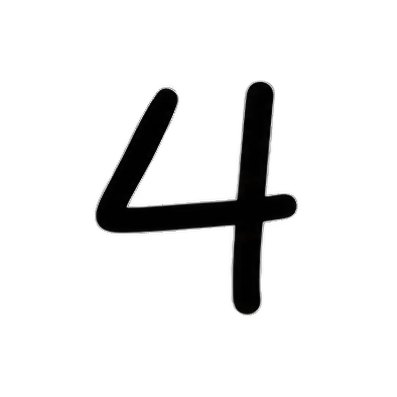
\includegraphics[width=2.2cm]{frame_01}};
  \draw[slate!50,line width=0.5pt] (9.15,3.55) rectangle (11.55,5.95);
  % ---------- right column ----------
  \node[anchor=north west,note,text width=3.0cm,visible on=<1-3>] at (11.9,5.95)
       {At $z_a$, the decoder draws a \textbf{4}.};
  \node[anchor=north west,note,text width=3.0cm,visible on=<2-3>] at (11.9,4.7)
       {Now slide $z$ along the line to~$z_b$\,\dots};
  \node[keybox,anchor=north west,text width=2.75cm,align=left,font=\footnotesize,visible on=<4>] at (11.9,6.05)
       {Every step decodes to a \textbf{real-looking} digit.
        \\[4pt] Remember the \textbf{gaps} from Part~1? The KL term filled them.};
  % ---------- filmstrip ----------
  \begin{scope}[visible on=<3->]
    \node[anchor=west,font=\scriptsize,text=slate] at (1.15,1.88) {decoded at each stop:};
    \foreach \k/\f/\xx in {1/01/5.0, 2/04/7.0, 3/07/9.0, 4/10/11.0}{
      \node[tile,minimum size=1.15cm] at (\xx,1.88) {};
      \node at (\xx,1.88) {\includegraphics[width=1.0cm]{frame_\f}};
      \node[badge,fill=navy,font=\tiny\bfseries,inner sep=1.2pt] at (\xx-0.575,2.455) {\k};}
    \foreach \xx in {5.7,7.7,9.7} \draw[fwd] (\xx,1.88) -- ++(0.6,0);
  \end{scope}
\end{canvas}
\end{frame}

% =================================================================
%  PAGE 3b — the walk, animated (frames from gen_images.py)
% =================================================================
\begin{frame}{Walking Through Latent Space}
\begin{canvas}
  \node[inner sep=0pt] at (8.0,4.15) {\animategraphics[autoplay,loop,palindrome,width=14cm]{10}{walk_}{01}{31}};
\end{canvas}
\end{frame}

% =================================================================
%  PAGE 4 — conditional VAE
%  diagram follows the reference: x, y -> encoder -> q(z|x,y) -> z -> decoder <- y
% =================================================================
\begin{frame}{Conditional VAE: Choosing What Comes Out}
\begin{canvas}
  % ---------- step 1: the problem, boxed ----------
  \node[rectangle,rounded corners=4pt,draw=slate!70,line width=0.8pt,fill=slate!6,anchor=south west,
        minimum width=6.8cm,minimum height=1.4cm] at (1.1,5.85) {};
  \node[anchor=north west,font=\footnotesize\bfseries,text=navy] at (1.25,7.17)
       {\textcolor{slate}{\xmark}\; Vanilla VAE: we can't pick the digit};
  \node[circle,fill=navy!8,draw=navy,line width=0.7pt,text=navy,minimum size=0.5cm,inner sep=0pt,font=\footnotesize] (pz) at (1.62,6.3) {$z$};
  \draw[fwd] (pz.east) -- (2.3,6.3);
  \decpoly{2.62}{6.3}{0.6}{0.62}{0.3}
  \draw[fwd] (2.92,6.3) -- (3.3,6.3);
  \foreach \d/\xx in {3b/3.6, 8b/4.1, 1/4.6}
    {\mthumb{\xx,6.3}{0.42}{mnist_\d}}
  \node[font=\footnotesize,text=slate] at (5.12,6.3) {\dots};
  \node[anchor=west,font=\scriptsize,text=slate] at (5.5,6.3) {random digit};
  % ---------- step 2: the fix, boxed ----------
  \begin{scope}[visible on=<2->]
    \node[rectangle,rounded corners=4pt,draw=teal,line width=0.8pt,fill=teal!6,anchor=south west,
          minimum width=6.8cm,minimum height=1.4cm] at (8.1,5.85) {};
    \node[anchor=north west,font=\footnotesize\bfseries,text=teal!80!black] at (8.25,7.17)
         {\cmark\; Conditional VAE (CVAE)};
    \node[anchor=west,font=\footnotesize,text=ink] at (8.3,6.3)
         {give the label $y$ to \textbf{both} halves};
  \end{scope}
  % ---------- step 3: the diagram ----------
  \begin{scope}[visible on=<3->]
    % inputs
    \node[font=\normalsize,text=ink] (x) at (1.55,4.9) {$x$};
    \node[ychip,focus on=<3>] (y1) at (1.55,3.7) {$y$};
    \draw[fwd] (x.east) -- (2.98,4.9);
    \draw[fwd] (y1.east) -- (2.98,3.7);
    % encoder
    \encpoly{3.85}{4.3}{1.6}{2.1}{1.0}
    \node[font=\footnotesize\bfseries,text=navy] at (3.85,4.3) {Encoder};
    \draw[fwd] (4.72,4.3) -- (5.3,4.3);
    % q(z|x,y) as a gaussian, with the sampled point
    \begin{scope}[shift={(6.6,3.7)}]
      \draw[slate!50,line width=0.5pt] (-1.25,0) -- (1.25,0);
      \fill[steel!12] plot[domain=-1.15:1.15,samples=41] (\x,{1.2*exp(-(\x*\x)/(2*0.38*0.38))}) -- cycle;
      \draw[steel,line width=0.8pt] plot[domain=-1.15:1.15,samples=41] (\x,{1.2*exp(-(\x*\x)/(2*0.38*0.38))});
      \draw[steel!70,line width=0.5pt,dash pattern=on 2pt off 1.5pt] (0,0) -- (0,1.2);
      \node[anchor=north,font=\scriptsize,text=steel] at (0,-0.04) {$\bm{\mu}$};
      \node[zdot] (s) at (0.45,0.6) {};
    \end{scope}
    \node[circle,fill=navy!8,draw=navy,line width=0.8pt,text=navy,minimum size=0.76cm] (z) at (8.85,4.5) {$z$};
    \draw[fwd] (s) to[out=65,in=165] (z.west);
    \node[font=\scriptsize,text=steel] at (7.72,5.2) {sampling};
    % decoder, with the label entering from below
    \draw[fwd] (z.east) -- (10.06,4.5);
    \node[ychip,focus on=<3>] (y2) at (9.55,3.25) {$y$};
    \draw[fwd] (y2.north) |- (10.06,4.05);
    \decpoly{10.9}{4.3}{1.6}{2.1}{1.0}
    \node[font=\footnotesize\bfseries,text=teal!70!black] at (10.9,4.3) {Decoder};
    \draw[fwd] (11.76,4.3) -- (12.36,4.3);
    \mthumb{12.95,4.3}{1.05}{mnist_7_m_recon}
    \node[lbl,text=ink] at (12.95,3.5) {$\hat{x}$};
  \end{scope}
  % labels under the blocks
  \node[anchor=north,font=\scriptsize,text=steel,visible on=<3->] at (3.85,2.9) {sees the image \emph{and} its label};
  \node[anchor=north,font=\scriptsize,text=teal!80!black,visible on=<3->] at (10.9,2.9) {draws the digit $y$ asks for};
  % ---------- step 4: the intuition ----------
  \node[mathbox,anchor=south west,text width=5.2cm,minimum height=1.3cm,align=left,font=\footnotesize,visible on=<4->] at (1.1,0.98)
       {The label $y$ says \textbf{\textcolor{teal!80!black}{which}} digit.
        \\[2pt] So $z$ only stores \textbf{\textcolor{navy}{how}} it is written.};
  % ---------- step 5: the payoff ----------
  \begin{scope}[visible on=<5->]
    \node[keybox,anchor=south west,text width=3.3cm,minimum height=1.3cm,align=left,font=\footnotesize] at (8.1,0.98)
         {$y=7$: \textbf{always a 7}, only the \emph{style} varies.};
    \foreach \f/\xx in {7_l/12.35, 7_m/12.9, 7_r/13.45}
      {\mthumb{\xx,1.63}{0.48}{mnist_\f}}
  \end{scope}
\end{canvas}
\end{frame}

% =================================================================
%  PAGE 5 — where VAEs are used (icon grid)
% =================================================================
% \usecase{centre x}{icon centre y}{icon macro}{colour}{title}{one line}
\newcommand{\usecase}[6]{%
  \fill[#4!8] (#1,#2) circle (0.85);
  \begin{scope}[shift={(#1,#2)},scale=1.12] #3{#4}{#4!30} \end{scope}
  \node[font=\normalsize\bfseries,text=#4!80!black] at (#1,{#2-1.2}) {#5};
  \node[font=\footnotesize,text=slate] at (#1,{#2-1.6}) {#6};}

\begin{frame}{Where VAEs Are Used}
\begin{canvas}
  \begin{scope}[visible on=<1->]
    \usecase{4.4}{6.05}{\icmagnifyingglass}{teal}{Anomaly Detection}{bad reconstruction $=$ something unusual}
    \usecase{11.6}{6.05}{\icflask}{navy}{Drug \& Molecule Design}{sample $z$ to get new molecules}
  \end{scope}
  \begin{scope}[visible on=<2->]
    \usecase{4.4}{2.95}{\icthumbsup}{steel}{Recommendation}{a latent ``taste'' for every user}
    \usecase{11.6}{2.95}{\icimages}{teal}{Data Augmentation}{decode extra training examples}
  \end{scope}
\end{canvas}
\end{frame}

% =================================================================
%  PAGE 6 — the VAE inside latent diffusion (Stable Diffusion)
%  columns: 5.64 image/noise, 7.44 encoder/U-Net, 9.09 latent, 10.84 decoder, 12.6 image
% =================================================================
\begin{frame}{How Diffusion Models Use a VAE}
\begin{canvas}
\begin{scope}[shift={(0,-0.25)}]
  % ---------- step 1: the VAE compresses ----------
  \begin{scope}[visible on=<1->]
    \node[anchor=west,font=\footnotesize\bfseries,text=slate] at (1.1,5.6) {1\enspace Compress};
    \person{5.64,5.6}{1.1}
    \node[anchor=north,font=\scriptsize,text=slate] at (5.64,4.85) {$512{\times}512{\times}3$};
    \draw[fwd] (6.34,5.6) -- (6.94,5.6);
    \encpoly{7.44}{5.6}{0.9}{1.2}{0.55}
    \node[anchor=north,font=\scriptsize,text=steel] at (7.44,4.85) {VAE encoder};
    \draw[fwd] (7.89,5.6) -- (8.54,5.6);
    \begin{scope}[shift={(8.59,5.1)},scale=1.4286] \lgrid{0}{11} \end{scope}
    \node[anchor=north,font=\scriptsize,text=navy] at (9.09,4.85) {latent};
    \node[anchor=west,font=\footnotesize,text=ink,align=left] at (9.85,5.6)
         {$64{\times}64{\times}4$\\[1pt]\textbf{\textcolor{navy}{48$\times$ fewer numbers}}};
  \end{scope}
  % ---------- step 2: diffusion works in that small space ----------
  \begin{scope}[visible on=<2->]
    \node[anchor=west,font=\footnotesize\bfseries,text=slate] at (1.1,3.0) {2\enspace Generate};
    \begin{scope}[shift={(5.14,2.5)},scale=1.4286] \lgrid{1}{23} \end{scope}
    \node[anchor=north,font=\scriptsize,text=slate] at (5.64,2.25) {noise};
    \draw[fwd] (6.14,3.0) -- (6.82,3.0);
    \unet{7.44}{3.0}
    \draw[navy,line width=0.7pt,->,>={Stealth[length=1.6mm]}] (7.84,3.42) .. controls (7.84,3.95) and (7.04,3.95) .. (7.04,3.42);
    \node[anchor=west,font=\scriptsize,text=navy] at (7.98,3.78) {$\times 50$};
    \node[chip,draw=slate!70,text=ink,font=\scriptsize,inner ysep=2pt] (prompt) at (7.44,1.55) {``a smiling face''};
    \draw[fwd] (prompt.north) -- (7.44,2.58);
    \draw[fwd] (8.06,3.0) -- (8.59,3.0);
    \begin{scope}[shift={(8.59,2.5)},scale=1.4286] \lgrid{0}{11} \end{scope}
    \node[anchor=north,font=\scriptsize,text=navy] at (9.09,2.25) {latent};
  \end{scope}
  % ---------- step 3: the VAE decoder paints the pixels ----------
  \begin{scope}[visible on=<3->]
    \draw[fwd] (9.59,3.0) -- (10.39,3.0);
    \decpoly{10.84}{3.0}{0.9}{1.2}{0.55}
    \node[anchor=north,font=\scriptsize,text=teal!80!black] at (10.84,2.25) {VAE decoder};
    \draw[fwd] (11.29,3.0) -- (11.94,3.0);
    \person{12.6,3.0}{1.1}
    \node[anchor=north,font=\scriptsize,text=slate] at (12.6,2.25) {new image};
  \end{scope}
\end{scope}
\end{canvas}
\end{frame}

% =================================================================
%  PAGE 7 — what is next for VAEs
% =================================================================
\begin{frame}{What's Next for VAEs}
\begin{canvas}
  % ---------- row 1 ----------
  \begin{scope}[visible on=<1->]
    \idea{1.1}{7.0}{Video generation}{Compressing space \emph{and} time, so AI can make whole clips.}
    \begin{scope}[shift={(1.95,5.875)},scale=1.3]
      \foreach \k/\c in {2/steel!25,1/steel!45,0/white}
        \filldraw[fill=\c,draw=steel,line width=0.6pt] ({-0.3+0.09*\k},{-0.22+0.09*\k}) rectangle ++(0.44,0.32);
      \fill[teal] (-0.13,-0.15) -- (-0.13,0.03) -- (0.02,-0.06) -- cycle;
    \end{scope}
    \idea{8.125}{7.0}{Robots that imagine}{Practising inside a learned latent world before acting.}
    \begin{scope}[shift={(8.975,5.875)},scale=1.3]
      \draw[slate,line width=0.6pt] (-0.15,0.05) -- (-0.15,0.16);
      \fill[teal] (-0.15,0.19) circle (0.035);
      \filldraw[fill=steel!20,draw=navy,line width=0.6pt,rounded corners=2pt] (-0.34,-0.3) rectangle (0.04,0.05);
      \fill[navy] (-0.22,-0.1) circle (0.035) (-0.08,-0.1) circle (0.035);
      \draw[navy,line width=0.5pt] (-0.22,-0.2) -- (-0.08,-0.2);
      \fill[slate!60] (0.1,0.08) circle (0.025) (0.16,0.15) circle (0.033);
      \filldraw[fill=white,draw=slate!70,line width=0.5pt] (0.26,0.27) circle (0.14);
      \fill[teal] (0.2,0.29) circle (0.027);
      \fill[navy] (0.3,0.22) circle (0.027);
      \fill[steel] (0.3,0.33) circle (0.027);
    \end{scope}
  \end{scope}
  % ---------- row 2 ----------
  \begin{scope}[visible on=<2->]
    \idea{1.1}{4.5}{New materials}{Sampling new crystals for better batteries and solar cells.}
    \begin{scope}[shift={(1.95,3.375)},scale=1.3]
      \draw[steel,line width=0.5pt] (-0.27,-0.3) rectangle (0.13,0.1) (-0.13,-0.16) rectangle (0.27,0.24);
      \draw[steel,line width=0.5pt] (-0.27,-0.3) -- (-0.13,-0.16) (0.13,-0.3) -- (0.27,-0.16)
                                    (0.13,0.1) -- (0.27,0.24) (-0.27,0.1) -- (-0.13,0.24);
      \foreach \p in {(-0.27,-0.3),(0.13,-0.3),(0.13,0.1),(-0.27,0.1),(-0.13,-0.16),(0.27,-0.16),(0.27,0.24),(-0.13,0.24)}
        \fill[navy] \p circle (0.045);
      \fill[teal] (0,-0.03) circle (0.07);
    \end{scope}
    \idea{8.125}{4.5}{Reading the brain}{Turning brain scans back into the images a person saw.}
    \begin{scope}[shift={(8.975,3.375)},scale=1.3]
      \foreach \i/\j/\v in {0/0/20,1/0/55,2/0/30,0/1/45,1/1/80,2/1/25,0/2/15,1/2/40,2/2/60}
        \fill[navy!\v] ({-0.4+\i*0.12},{-0.18+\j*0.12}) rectangle ++(0.11,0.11);
      \draw[slate,line width=0.5pt,->,>={Stealth[length=1mm]}] (-0.02,0) -- (0.07,0);
      \person{0.24,0}{0.28}
    \end{scope}
  \end{scope}
  % ---------- closing ----------
  \begin{scope}[visible on=<3->]
    \fill[teal!6,rounded corners=4pt] (1.1,0.98) rectangle (14.9,1.78);
    \draw[teal,line width=1.0pt,rounded corners=4pt] (1.1,0.98) rectangle (14.9,1.78);
    \node[font=\footnotesize,text=ink] at (8.0,1.38)
         {\textbf{\textcolor{steel}{compress}} $\rightarrow$ \textbf{\textcolor{navy}{smooth}} $\rightarrow$
          \textbf{\textcolor{teal!80!black}{sample}}: the same recipe, aimed at new problems.};
  \end{scope}
\end{canvas}
\end{frame}

% =================================================================
%  CLOSING SLIDE — just "Thank you"
% =================================================================
{
\setbeamertemplate{footline}{}
\begin{frame}[plain]
\begin{tikzpicture}[remember picture,overlay,shift={(current page.south west)}]
  \node[text=navy,font=\fontsize{30}{33}\fontseries{eb}\selectfont] at (8,4.5) {Thank You};
\end{tikzpicture}
\end{frame}
}

\end{document}
